\newpage
\textbf{Ejemplo 11}\newline
	Una aceptación bancaria por 80 millones COP con fecha de vencimiento el 17 de diciembre de 1999 es adquirida en 22 de julio de 1999 por un primer inversionista con una tasa del de 28\% período 28 días vencidos y es cedida a un segundo inversionista el 14 de octubre de 1999. Si el segundo inversionista desea ganarse el 32\% período días vencido utilice un año de 360 (año de 360 días) \\
	¿Cuál es la ganancia en pesos del primer inversionista? \\
	¿Cuál es la rentabilidad periódica días vencido del primer inversionista?\\
	

	\textbf{Solución.}
	\begin{center}
		\renewcommand{\arraystretch}{1.5}% Margenes de las celdas
		%Creación de la cuadricula
	\begin{longtable}[H]{|p{0.33\linewidth}|p{0.33\linewidth}|p{0.33\linewidth}|}
		\hline
		\rowcolor[HTML]{FFB183} 
		\multicolumn{3}{|c|}{\cellcolor[HTML]{FFB183}\textbf{1. Asignación período focal}}   \\ \hline
		\multicolumn{3}{|c|}{$pf : 0 pdv$} \\ \hline
		\rowcolor[HTML]{FFB183}
		\multicolumn{3}{|c|}{\cellcolor[HTML]{FFB183}\textbf{2. Declaración de variables}}\\
		\hline
		%%%%%%%%%% INICIO SUBTITULO
		\multicolumn{1}{|c|}{\cellcolor[HTML]{FFB183}\textbf{Valores monetarios}}    & 
		\multicolumn{1}{|c|}{\cellcolor[HTML]{FFB183}\textbf{Valores no monetarios}} &
		\multicolumn{1}{|c|}{\cellcolor[HTML]{FFB183}\textbf{Incógnitas}}  \\ \hline
		%%%%%%%%%% FIN SUBTITULO
		
		& $i_{1} = 28 \% pdv$ &  $P_{C2} - P_{C1} = ? $ \\
		& $i_{2} = 32\% pdv \hspace{0.3cm} $ &  \\ 
		&$ n_{1} = \frac{145}{365} = 0,4028 \ pdv $  & \\
		&$ n_{2} = \frac{63}{365} = 0.175 \ pdv $ & \\
		&$ n_{3} = 0 \ pdv $ & \\
		\hline
	
		%%%%%%%%%% FIN DE MATEMÁTICAS
		%%%%% FIN DECLARACIÓN DE VARIABLES
		
		
	%%%%% INICIO FLUJO DE CAJA
	\rowcolor[HTML]{FFB183}
	\multicolumn{3}{|c|}{\cellcolor[HTML]{FFB183}\textbf{3. Diagrama de flujo de caja}} \\ \hline
	\multicolumn{3}{|c|}{ 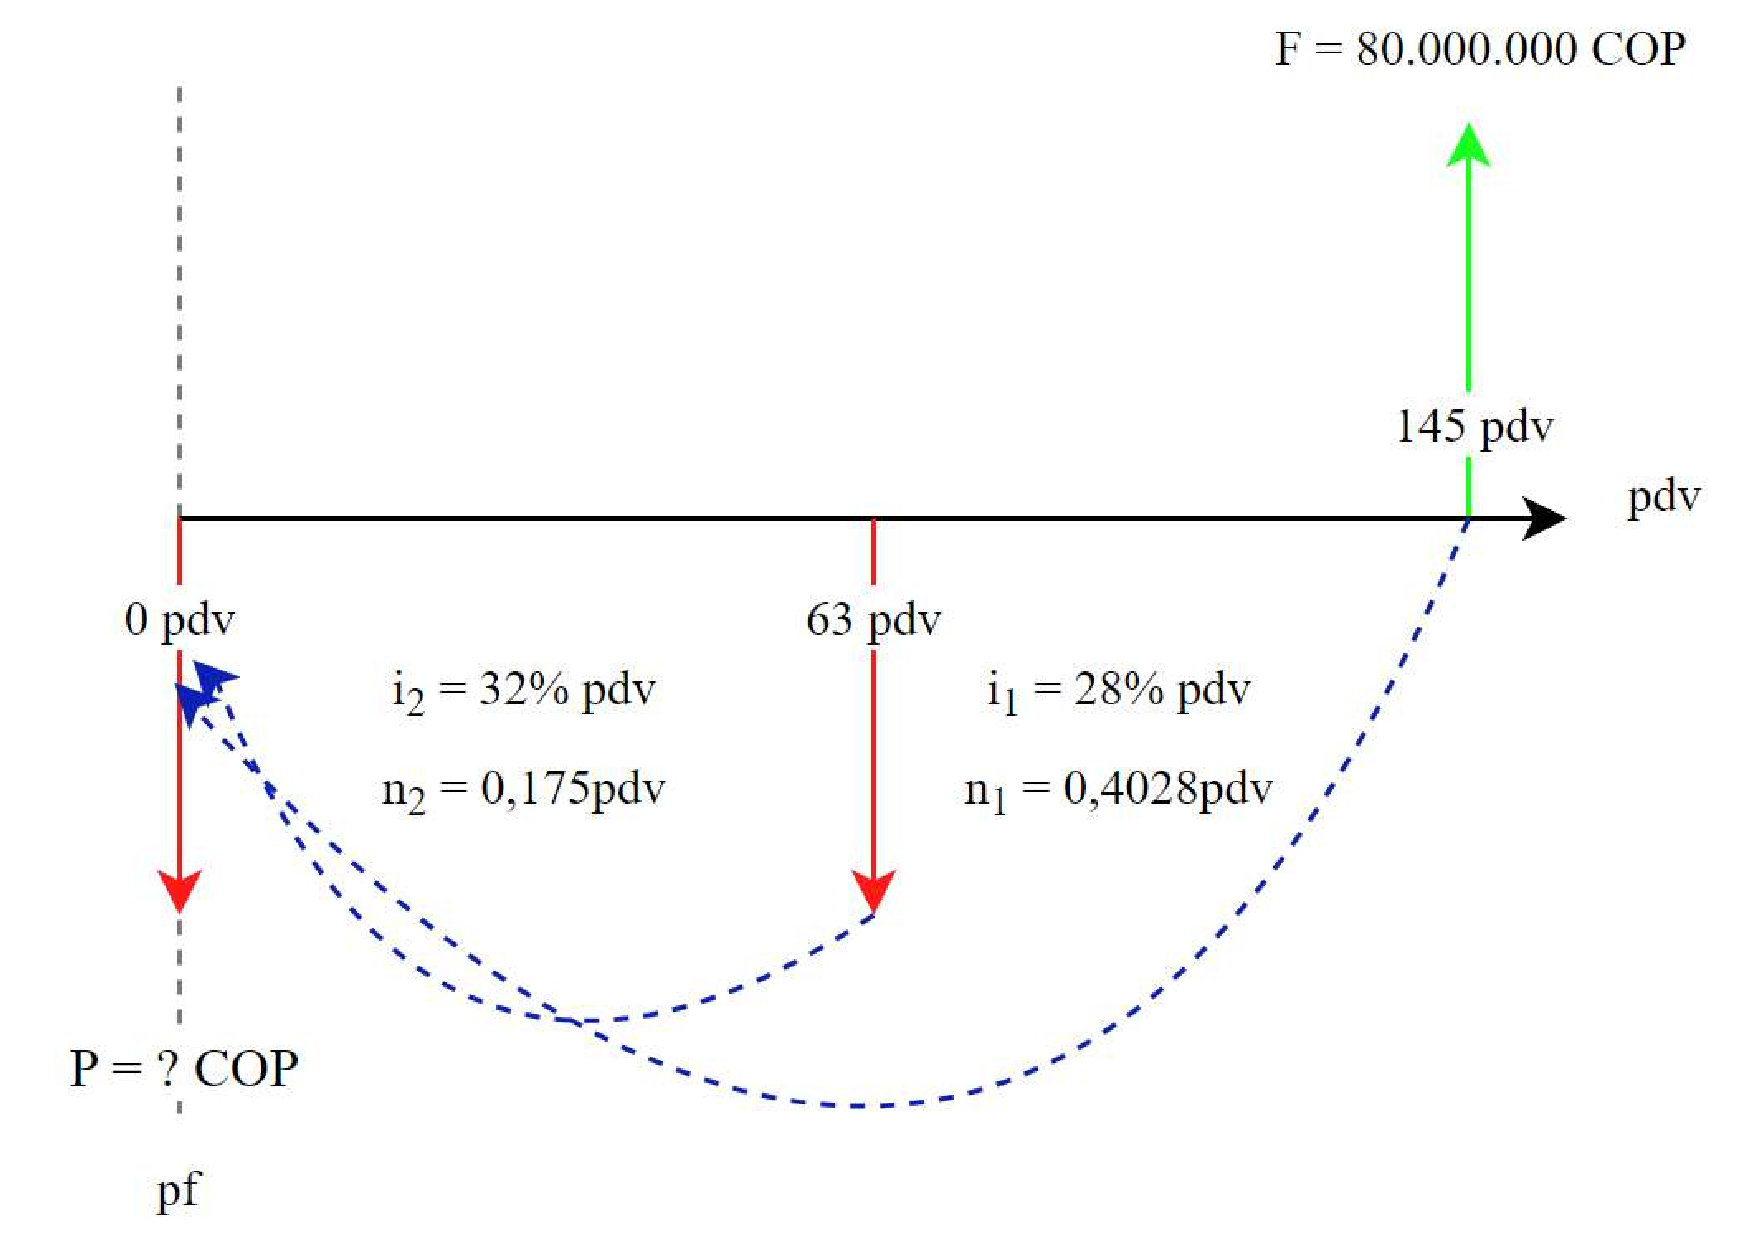
\includegraphics[trim=-5 -5 -5 -5 , scale=0.55, width=16.4 cm, height = 10.5 cm]{3_Capitulo/img/ejemplos/11/capitulo3ejercicio11.pdf} } \\ \hline
	
	\rowcolor[HTML]{FFB183}
	\multicolumn{3}{|c|}{\cellcolor[HTML]{FFB183}\textbf{4. Declaración de fórmulas}} \\ \hline
	
	\multicolumn{3}{|c|}{$P=F(1+i)^{-n}$\hspace{35pt}\textit{Valor presente}
		\hspace{0.3cm}}\\ \hline
	%%%%%%%%%% FIN MATEMÁTICAS
	%%%%% INICIO DESARROLLO MATEMÁTICO
	\rowcolor[HTML]{FFB183}
	%%%%%%%%%%INICIO TITULO
	\multicolumn{3}{|c|}{\cellcolor[HTML]{FFB183}\textbf{5. Desarrollo matemático}} \\ \hline
	%%%%%%%%%% FIN TITULO
	%%%%%%%%%% INICIO MATEMÁTICAS
	\multicolumn{3}{|c|}{$P_c =   80{.}000{.}000 COP (1+0,28)\frac{-145}{360}$ =   72{.}428{.}283,64 COP }
	\\ 
	\multicolumn{3}{|c|}{\hspace{3pt} $P_c \equiv$   72{.}428{.}284 COP \hspace{3pt}\textit{Ecuación de equivalencia}}
	\\
	\multicolumn{3}{|c|}{$V_c =   80{.}000{.}000 COP(1+0,32)\frac{-63}{360} =    76{.}206{.}067 COP$ \hspace{3pt}\textit{Ecuación de equivalencia}}
	\\ 
	\multicolumn{3}{|c|}{$P_c =  V_{c} - P_{c} COP  = 76{.}206{.}067 - 72{.}428{.}284 $}
	\\
	\multicolumn{3}{|c|}{$ =   3{.}777{.}738 COP  $ \hspace{3pt}\textit{Ecuación de equivalencia}}
	\\
	\hline
	%%%%%%%%%% FIN MATEMÁTICAS
	%%%%% FIN DESARROLLO MATEMÁTICO
	
	\rowcolor[HTML]{FFB183}
	\multicolumn{3}{|c|}{\cellcolor[HTML]{FFB183}\textbf{6. Respuesta}} \\ \hline    
	
	\multicolumn{3}{|c|}{$V_{c} - P_{c} =  3{.}777{.}783 COP  $} \\ \hline
	\end{longtable}
\end{center}

	